\section{Характеристический метод для сеток плохого качества}

\subsection{Необходимость разработки метода}

Одной из принципиальных проблем, с которыми сталкивается метод характеристик на сетках из тетраэдров при попытке расчета им реальных задач, является низкое качество сеток, создаваемых стандартными генераторами сеток. Данный вопрос практически всегда остается за рамками в любых публикациях по теме сеточно-характеристических методов, так как не связан непосредственно с конструированием самого метода. Тем не менее, для практики эта проблема крайне важна, поэтому остановимся на ней подробнее.

Если подходить к вопросу формально, то сеточно-характеристический метод может использоваться на любой сетке из тетраэдров. Однако, как было рассмотрено выше, для сеток из тетраэдров имеет место ограничение на шаг по времени, аналогичное курантовскому шагу для равномерной прямоугольной сетки. Так для каждого узла сетки:

\begin{equation}
\tau \le \frac{\min(h)}{\max(|\lambda|)},
\end{equation}

где $\min(h)$ -- минимальная высота тетраэдра, в которые входит данный узел, $\max(|\lambda|)$ -- максимальное по модулю собственное число матрицы $\mathbf A$ для данного узла.

С практической точки зрения крайне нежелательна ситуация, когда $\tau$ оказывается малым для отдельных узлов сетки, так как это накладывает ограничения на шаг по времени для всей сетки. Разумеется, необходимо различать случай, когда малый шаг по времени продиктован объективными требованиями высокого разрешения по времени и пространству, и случай, когда он является нежелательным следствием тех или иных проблем. В данный момент мы сосредоточимся на втором случае.

В таблице \ref{tbl:mesh-stats-summary} приведены данные по сеткам из тетраэдров, созданных в кубе с ребром 10 с помощью различных генераторов. Во всех случаях было задано значение мелкости сетки $h_* = 0.25$. В идеальном случае была бы построена сетка из правильных тетраэдров одинакового размера с высотами ровно равными $h_*$. Если такое оказалось бы возможно, то шаг по времени точно соответствовал бы ожидаемому $\tau_* \le h_* / \lambda$ и зависел бы только от реологии среды (значения $\lambda$). Очевидно, что в случае реальной геометрии построить сетку полностью из правильных тетраэдров одного размера невозможно, поэтому следует ожидать появления тетраэров размером несколько больше или меньше, чем заданный, а также тетраэдров с искажениями относительно правильной формы. Полученная в итоге минимальная высота тетраэдра определяет шаг по времени для всей сетки $\tau \le \min(h) / \lambda$. В связи с этим логично ввести критерий качества сетки в следующем виде:

\begin{equation}
q = \frac{\min(h)}{h_*},
\end{equation}

где $h_*$ -- заданная желаемая мелкость сетки, а $\min(h)$ -- минимальная высота в сетке, фактически выданной генератором.

Для идеальной сетки $q = 1$. В случае не слишком больших отклонений от единицы сетку можно считать "достаточно хорошей" для расчёта. Однако, как видно из \ref{tbl:mesh-stats-summary}, на практике даже для простейшей геометрии $q$ находится в диапазоне $0.00065 \le q \le 0.126$. Это приводит к неоправданному падению шага по времени на 1-3 порядка и, соответственно, к необоснованному росту требуемого объема вычислений также на 1-3 порядка. Приведенные гистограммы распределения высот тетраэдров в полученных сетках показывают, что проблема не связана с наличием единичных вырожденных тетраэдров, а носит систематический характер. Эксперименты с объектами более сложной геометрии показывают еще худшие результаты по качеству сетки.

Причиной такого низкого качества сеток является тот факт, что все существующие генераторы сеток ориентированы на построение сеток для метода конечных элементов. Для МКЭ критерии качества сетки совершенно иные -- размеры тетраэдров не важны, для эффективной работы метода требуется, чтобы их углы были максимально близки к правильным, а линейные размеры при этом могут быть любыми. Соответственно, ориентированные на МКЭ алгоритмы построения сеток оказываются неэффективными с точки зрения сеточно-характеристического метода.

Очевидным способом решения данной проблемы может быть разработка алгоритмов построения сеток, ориентированных на улучшения качества в терминах сеточно-характеристического метода. Однако в данной работе предлагается другой подход -- модификация метода для обеспечения эффективной работы на сетке низкого качества. Данный подход, как будет рассмотрено ниже, может применяться не только для решения проблемы малого шага по времени из-за низкого качества изначальной сетки, но и в случае деградации шага по времени из-за вырождения сетки в зоне больших деформаций.

\begin{table}[h]
\centering
\begin{tabular}{|c|c|c|c|}
\hline
Генератор & Заданное $H$ & Полученное $\min(H)$ & Полученное $\max(H)$ \\
\hline
gmsh & 0.25 & 0.000845531 & 0.307492 \\
tetgen & 0.25 & 0.0315793 & 0.279029 \\
Ani3D & 0.25 & $1.08e^{-8}$ & 3.63429 \\
Ani3D + косметика & 0.25 & 0.000162557 & 3.7205 \\
\hline
\end{tabular}
\caption{Качество сеток, созданных различными генераторами в кубе с ребром 10.}
\label{tbl:mesh-stats-summary}
\end{table}


\begin{figure}[htp]
\centering
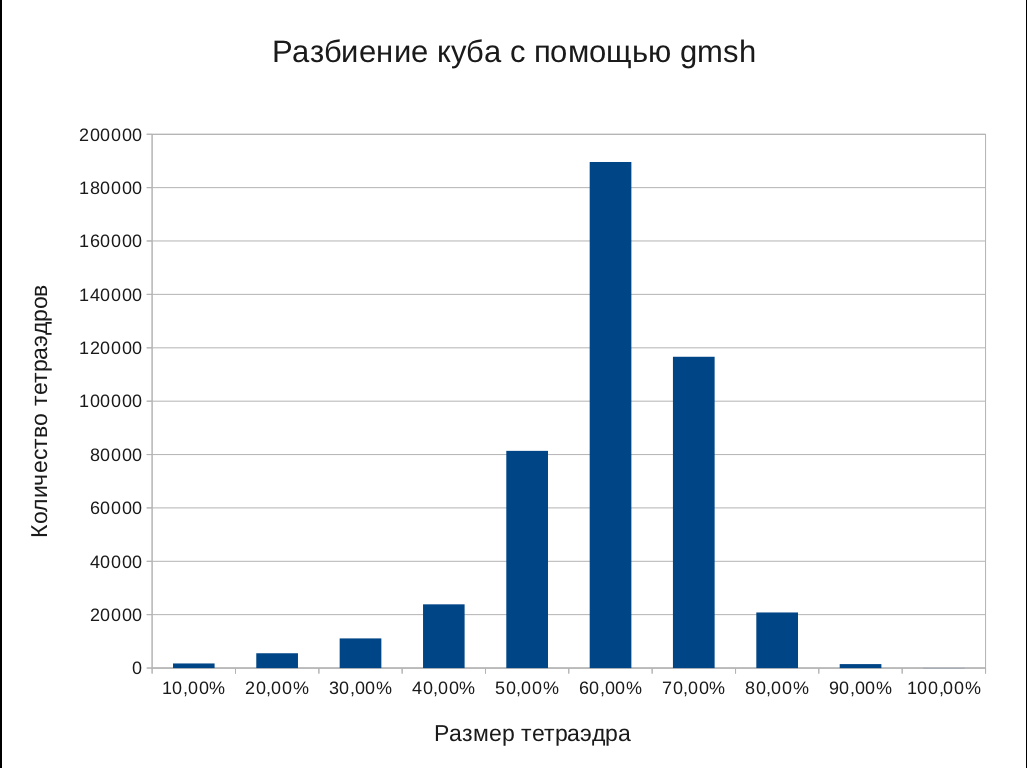
\includegraphics[width=0.8\textwidth]{png/gmsh-stats.png}
\caption{Сетка в кубе, созданная с помощью gmsh. Распределение тетраэдров по размеру.}
\end{figure}

\begin{figure}[htp]
\centering
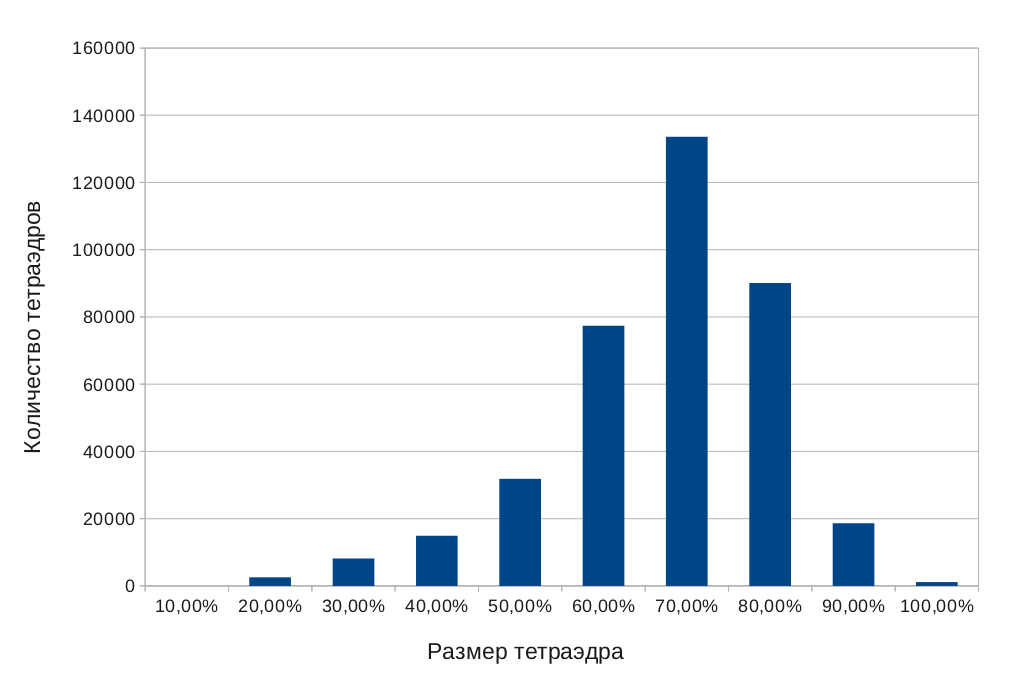
\includegraphics[width=0.8\textwidth]{png/tetgen-stats.png}
\caption{Сетка в кубе, созданная с помощью tetgen. Распределение тетраэдров по размеру.}
\end{figure}

\begin{figure}[htp]
\centering
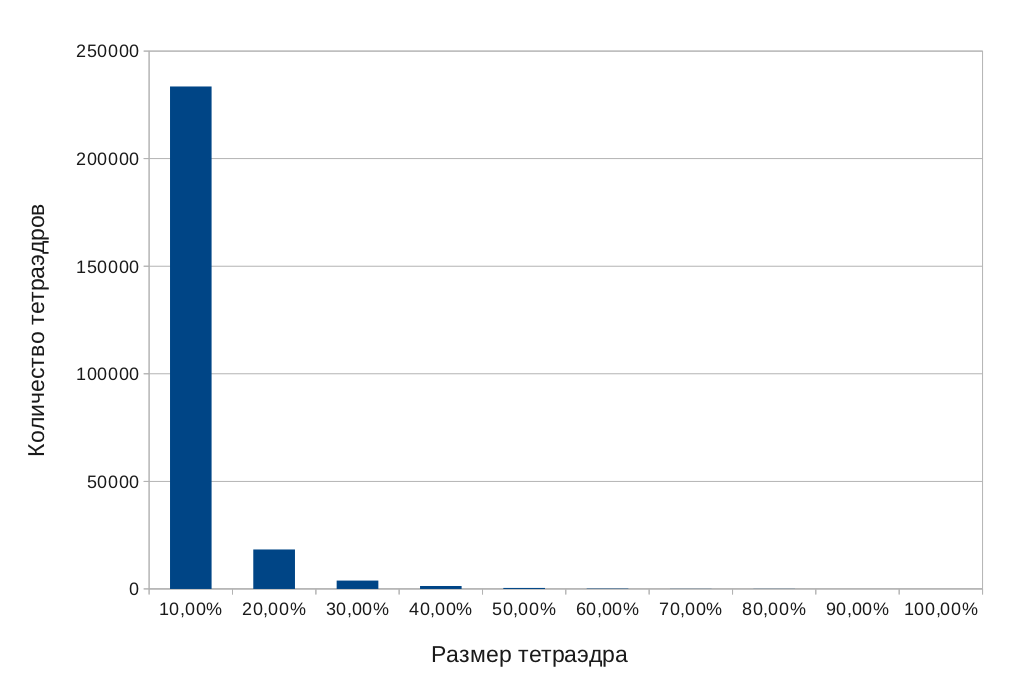
\includegraphics[width=0.8\textwidth]{png/ani3d-stats.png}
\caption{Сетка в кубе, созданная с помощью Ani3D. Распределение тетраэдров по размеру.}
\end{figure}

\begin{figure}[htp]
\centering
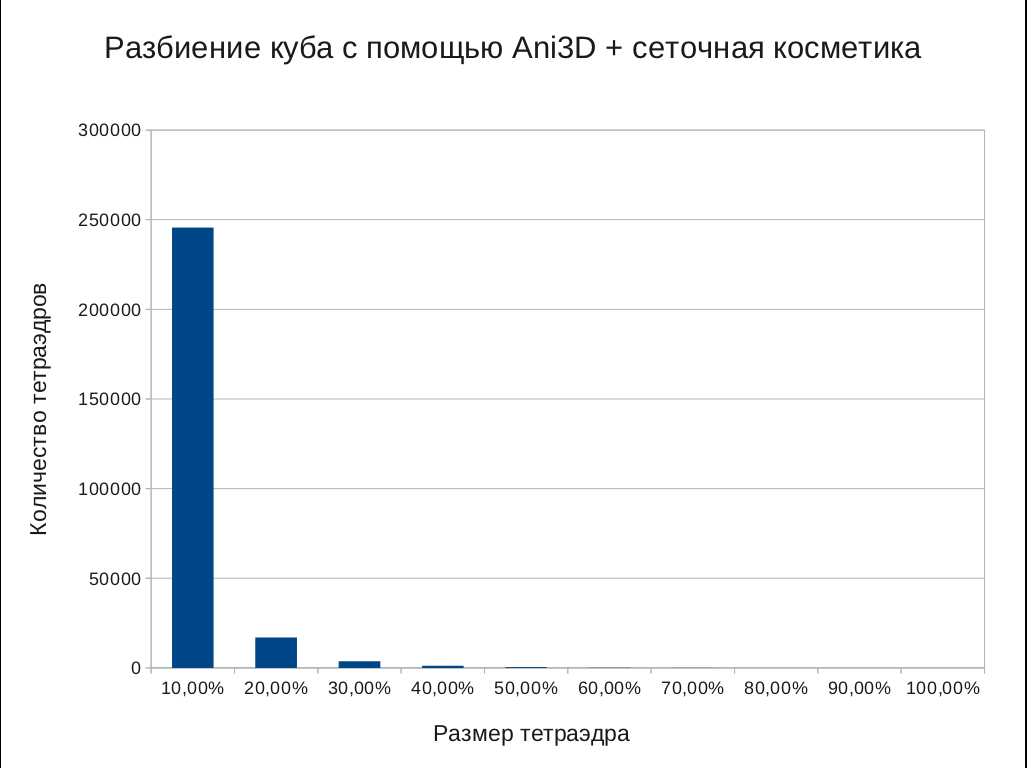
\includegraphics[width=0.8\textwidth]{png/ani3d-improved-stats.png}
\caption{Сетка в кубе, созданная с помощью Ani3D с применением сеточной косметики. Распределение тетраэдров по размеру.}
\end{figure}

\clearpage
\newpage

\subsection{Метод для одномерной задачи}

\subsubsection{Конструирование метода}

Рассмотрим одномерное уравнение переноса

\begin{equation}
\frac{\partial{u}}{\partial{t}} + \lambda \frac{\partial{u}}{\partial{x}} = 0, \lambda \ne const.
\end{equation}

Введем в области интегрирования разностную сетку и обозначим $u_m^n = u(t^n, x_m)$. Обратим внимание, что мы изначально предполагаем неравномерность сетки. Это соответствует как случаю с изначально сеткой низкого качества, так и случаю больших деформаций и вырождения сетки. Кроме того, мы рассматриваем случай разных значений $\lambda$ в разных точках расчетной области. Такая ситуация имеет место, если среда изначально неоднородная или если большие деформации вызвали значительное локальное изменение плотности в точке.

Особенностью предлагаемого метода является тот факт, что на данном этапе не будем выбирать фиксированный сеточный шаблон. Необходимые точки на предыдущем временном слое, по которым выполняется реконструкция значений на следующем шаге по времени, будут определяться в ходе вычислений отдельно для каждой рассчитываемой точки, исходя из локальных свойств решения в ней.

Предположим, что из тех или иных соображений был выбран шаг по времени $\tau$, такой что характеристика из точки $u_m^n$ не попадает в отрезок $(u_{m-1}^n; u_{m+1}^n)$.

\begin{figure}[h]
\center{\includegraphics[width=0.5\textwidth]{eps/gcm-idea.eps}}
\caption{Характеристика при большом шаге $\tau$.}
\end{figure}

В этом случае найдем тот отрезок $(u_{m-k-1}^n; u_{m-k}^n)$, в котором выпущенная характеристика пересекает временной слой $n$ (точка $x^*$ на рисунке). Обозначим:
\begin{eqnarray}
x_{m-k} - x_{m-k-1} = h_k,\nonumber\\
x_m - x^* = \lambda \tau = l_0,\nonumber\\
x_m - x_{m-k} = l_k.
\end{eqnarray}

Нормируя $l_k$ и $l_0$ на $h_k$ получаем:
\begin{eqnarray}
q_0 = l_0 / h_k = \lambda \tau / h_k = \sigma,\nonumber\\
q_k = l_k / h_k,
\end{eqnarray}
где $\sigma$ -- аналог классического числа Куранта для равномерной сетки.

Рассмотрим простейший случай линейной интерполяции значения в точке $u_*^n$ по точкам  $u_{m-k-1}^n$ и $u_{m-k}^n$. Получаем для значения на новом временном слое $u_m^{n+1}$ следующее выражение:
\begin{eqnarray}
\label{newmethod_1d_scheme}
u_m^{n+1} = u_*^n = (q_k + 1 - q_0) u_{m-k}^n + (q_0 - q_k) u_{m-k-1}^n.
\end{eqnarray}

\clearpage
\newpage

\subsubsection{Исследование метода}

Чтобы найти порядок аппроксимации по времени и по пространству используем разложение $u_{m+\mu}^{n+\nu}$ в ряд Тейлора. Обозначим:
\begin{eqnarray}
q_0 - q_k = \sigma_k,\nonumber\\
\frac{h_k}{l_0} = \alpha,\nonumber\\
\frac{l_k}{l_0} = \beta,
\end{eqnarray}
где очевидно $\alpha < 1, \beta < 1$.

Раскладывая \ref{newmethod_1d_scheme} в ряд Тейлора в окрестности $u = u_m^n$ до второго порядка малости получаем:
\begin{eqnarray}
u + u_\tau \tau + u_{\tau\tau} \frac{\tau^2}{2} = (1 - \sigma_k) (u - l_k u_x + u_{xx} \frac{l_k^2}{2}) + \sigma_k (u - (l_k+h_k) u_x + u_{xx} \frac{(l_k+h_k)^2}{2}) \nonumber\\
u_\tau \tau + u_{\tau\tau} \frac{\tau^2}{2} = (1 - \sigma_k) (- l_k u_x + u_{xx} \frac{l_k^2}{2}) + \sigma_k (- (l_k+h_k) u_x + u_{xx} \frac{(l_k+h_k)^2}{2}) \nonumber\\
u_\tau \tau + u_{\tau\tau} \frac{\tau^2}{2} = - u_x ( (1 - \sigma_k) l_k + \sigma_k (l_k+h_k) ) + \frac{u_{xx}}{2} ( (1 - \sigma_k) l_k^2 + \sigma_k (l_k+h_k)^2 ) \nonumber\\
u_\tau \tau + u_x  ( l_0 ) = - u_{\tau\tau} \frac{\tau^2}{2} + \frac{u_{xx}}{2} ( l_k^2 + 2 \sigma_k l_k h_k + \sigma_k h_k^2 ) \nonumber\\
u_\tau \tau + u_x  \lambda \tau = - u_{\tau\tau} \frac{\tau^2}{2} + \frac{u_{xx}}{2} ( l_k (l_k + \sigma_k h_k) + \sigma_k h_k (l_k + h_k) ) \nonumber\\
u_\tau \tau + u_x  \lambda \tau = - u_{\tau\tau} \frac{\tau^2}{2} + \frac{u_{xx}}{2} ( l_k l_0  + \sigma_k h_k l_0 (\alpha + \beta) ) \nonumber\\
u_\tau + u_x  \lambda = - u_{\tau\tau} \frac{\tau}{2} + \frac{u_{xx}}{2} \lambda ( l_k  + \sigma_k h_k (\alpha + \beta) ) \nonumber\\
u_\tau + u_x  \lambda = O(\tau) + O (h)
\end{eqnarray}

Таким образом, схема имеет первый порядок по времени и по пространству. Этого следовало ожидать, так как используемая линейная интерполяция имеет первый порядок точности.

Для исследования устойчивости воспользуемся методом Фурье. Рассмотрим $u_m^n = v^n e^{im\phi}$. Подставив его в \ref{newmethod_1d_scheme} получим:
\begin{eqnarray}
v^{n+1} e^{im\phi} = (q_k + 1 - q_0) v^{n} e^{i(m-k)\phi} + (q_0 - q_k) v^{n} e^{i(m-k-1)\phi} \nonumber\\
v^{n+1} e^{im\phi} = v^{n} e^{im\phi} ((q_k + 1 - q_0) e^{-ik\phi} + (q_0 - q_k) e^{-i(k+1)\phi} \nonumber\\
u_m^{n+1} = u_m^n ((q_k + 1 - q_0) e^{-ik\phi} + (q_0 - q_k) e^{-i(k+1)\phi}).
\end{eqnarray}

Таким образом, оператор перехода от слоя $n$ к слою $n+1$ имеет вид:
\begin{eqnarray}
\lambda = e^{-ik\phi} ( 1 + (q_k - q_0) (1 - e^{-i\phi}) ).
\end{eqnarray}

Необходимое условие устойчивости Неймана:
\begin{eqnarray}
|\lambda|^2 \le 1 \nonumber\\
| 1 + (q_k - q_0) (1 - e^{-i\phi}) |^2 \le 1 \nonumber\\
| 1 + (q_k - q_0) (1 - \cos(\phi)) + i(q_k - q_0)\sin(\phi) |^2 \le 1 \nonumber\\
( 1 + (q_k - q_0) (1 - \cos(\phi)))^2 + ((q_k - q_0)\sin(\phi))^2 \le 1 \nonumber\\
( 1 + q_k - q_0)^2 - 2 ( 1 + q_k - q_0)(q_k - q_0) \cos(\phi) + (q_k - q_0)^2 \le 1 \nonumber\\
1 + 2 (q_k - q_0) + 2 (q_k - q_0)^2 - 2 ( 1 + q_k - q_0)(q_k - q_0) \cos(\phi) \le 1 \nonumber\\
(q_k - q_0)^2 - (q_k - q_0) ( 1 + q_k - q_0 ) \cos(\phi) + (q_k - q_0) \le 0 \nonumber\\
(q_k - q_0)(q_k - q_0 + 1)(1 - \cos(\phi)) \le 0 \nonumber\\
(q_k - q_0)(q_k - q_0 + 1) \le 0
\end{eqnarray}

Отсюда получаем
\begin{eqnarray}
-1 \le q_k - q_0 \le 0, \nonumber\\
q_k \le q_0 \le q_k + 1.
\end{eqnarray}

Таким образом, схема устойчива при 
\begin{eqnarray}
k \le \sigma \le k+1.
\end{eqnarray}

Так как все коэффициенты схемы неотрицательны, то она также является монотонной в соответствии с критерием Фридрихса.

Полученное условие де-факто эквивалентно условию попадания характеристики в отрезок, по которому производится интерполяция. Если для реконструкции решения используется интерполяция более высоких порядков, то необходимый сеточный шаблон будет расширяться. Например, для интерполяции второго порядка необходимо использовать три точки на временном слое $n$. В этом случае можно выбрать любой из трехточечных шаблонов, включающих в себя $x^*$ -- $(u_{m-k-2}^n; u_{m-k}^n)$ или $(u_{m-k-1}^n; u_{m-k+1}^n)$. В общем случае, в соответствии с \cite{magomedov}, все схемы с порядком аппроксимации выше первого не будут монотонны.

\clearpage
\newpage

\subsubsection{Тестирование метода}

На рис. \todo{N} приведены результаты тестирования описанной схемы. Рассматривалась задача распада разрыва. Использовалась равномерная сетка по пространству. Приведены графики для расчетов с $\lambda \tau / h = 1.0$ (классический шаблон "уголок" с курантовским шагом) и $\lambda \tau / h = 1.5$ (описанная выше схема).

\begin{figure}[htp]
\centering
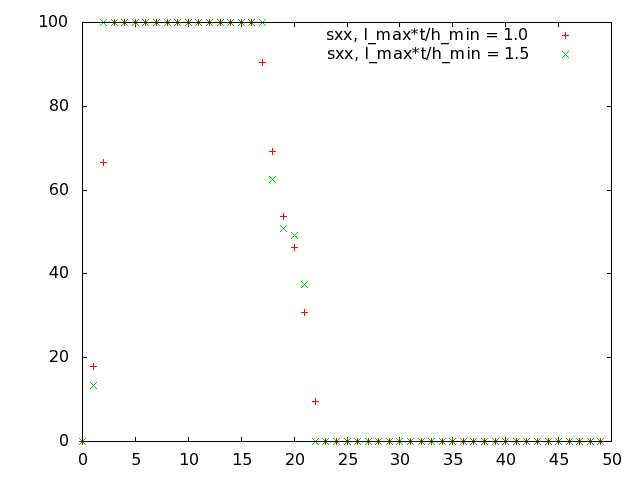
\includegraphics[width=0.6\textwidth]{png/big-sigma-test-results-1d/snap-1.png}
\caption{1-ый шаг по времени.}
\end{figure}

\begin{figure}[htp]
\centering
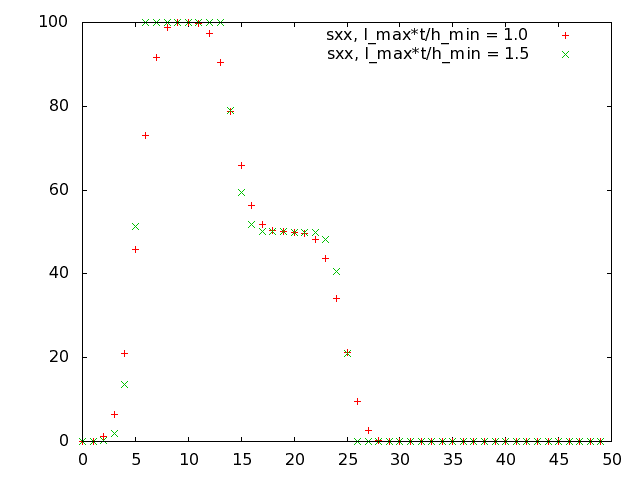
\includegraphics[width=0.6\textwidth]{png/big-sigma-test-results-1d/snap-3.png}
\caption{3-ий шаг по времени.}
\end{figure}

\begin{figure}[htp]
\centering
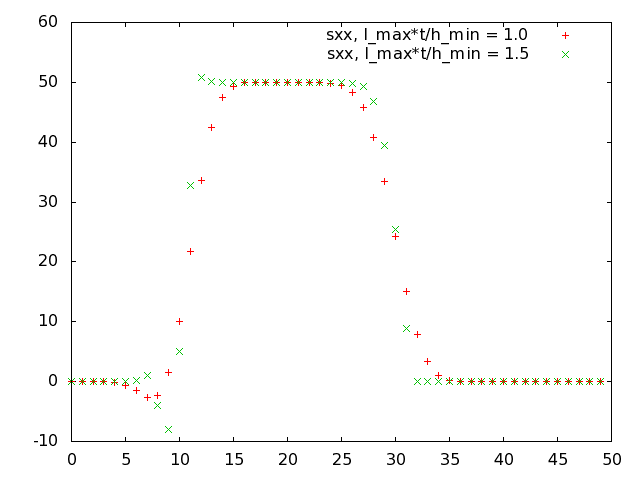
\includegraphics[width=0.6\textwidth]{png/big-sigma-test-results-1d/snap-6.png}
\caption{6-ой шаг по времени.}
\end{figure}

\begin{figure}[htp]
\centering
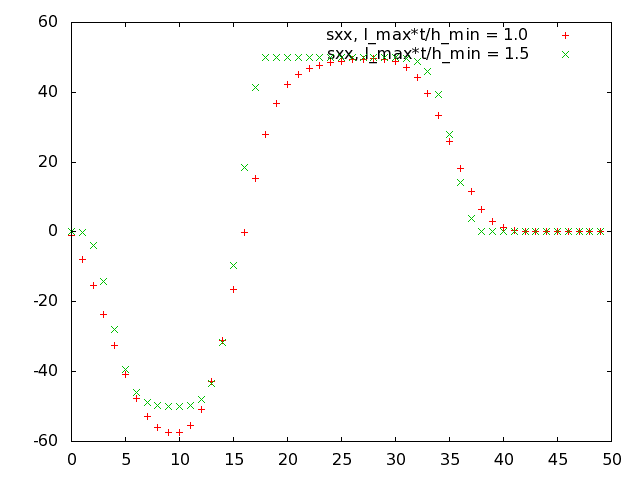
\includegraphics[width=0.6\textwidth]{png/big-sigma-test-results-1d/snap-9.png}
\caption{9-ый шаг по времени.}
\end{figure}

\begin{figure}[htp]
\centering
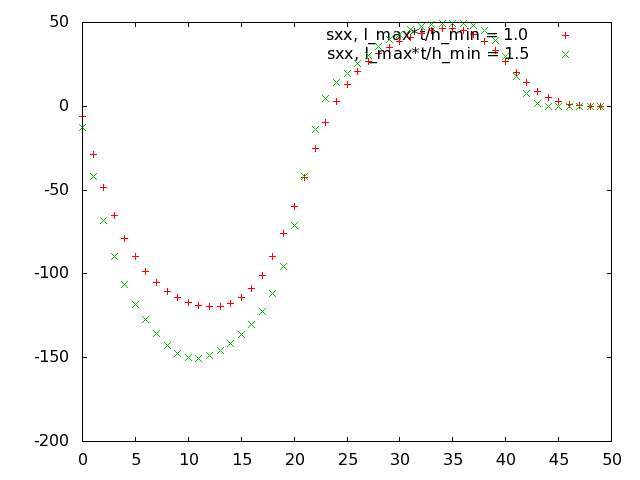
\includegraphics[width=0.6\textwidth]{png/big-sigma-test-results-1d/snap-12.png}
\caption{12-ый шаг по времени.}
\end{figure}

\clearpage
\newpage

\subsection{Метод для трёхмерной задачи}

\subsubsection{Конструирование метода на неструктурированной сетке}

\begin{figure}[htp]
\centering
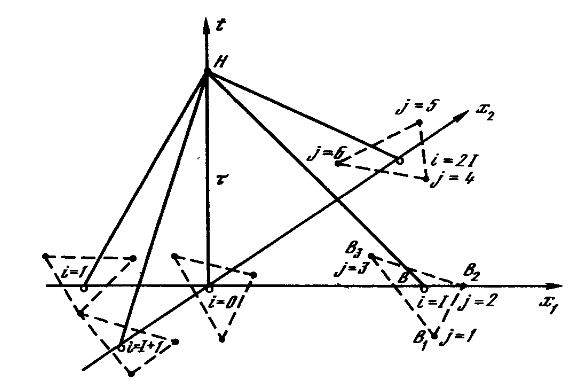
\includegraphics[width=0.6\textwidth]{png/characteristics-2d-triangles-inner.png}
\caption{Расчет внутреннего узла.}
\end{figure}

\subsubsection{Расчёт внутренних узлов}

\todo{Расчёт приграничных узлов и грабли при этом. Вылетание части характеристик.}

\begin{figure}[htp]
\centering
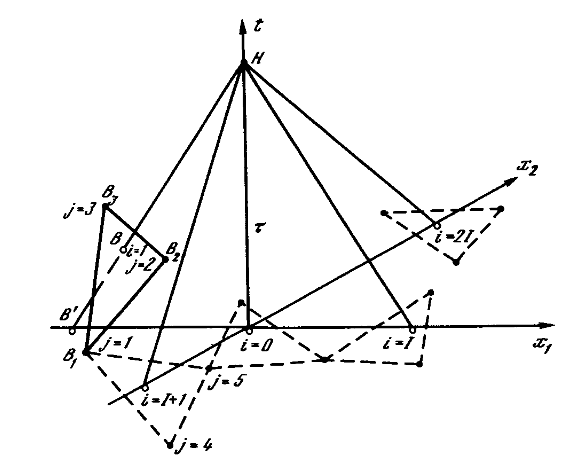
\includegraphics[width=0.6\textwidth]{png/characteristics-2d-triangles-semi-border.png}
\caption{Расчет узла, близкого к границе.}
\end{figure}


\subsubsection{Расчёт граничных и контактных узлов}

\begin{figure}[htp]
\centering
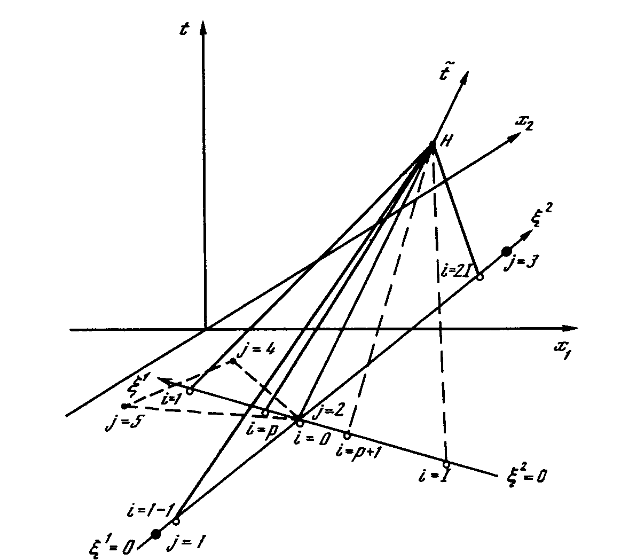
\includegraphics[width=0.6\textwidth]{png/characteristics-2d-triangles-border.png}
\caption{Расчет граничного узла.}
\end{figure}

\clearpage
\newpage

\subsubsection{Использование совместно с движущейся сеткой при больших деформациях}

\clearpage
\newpage

\subsubsection{Исследование метода}

\todo{Аппроксимация, устойчивость, монотонность}

